\section{Models}\label{sec:model-examples}
This section shows the IOGG and IOSTS for each model example and the case study. There are four examples; the last one shows the example can only modelled by violating the constraints in section~\ref{sec:constraints}. 

\subsection{Example 1: boardgame}
The boardgame is the running example of which the IOSTS and IOGG are given in Figures~\ref{fig:example_sts} and \ref{fig:example_groove} respectively. In order to be consistent with the GG variable definition, the two $Player$ and $Die$ nodes receive the flags $\mathit{var1, var2, var3}$ respectively, representing the variable labels.

\subsection{Example 2: farmer-wolf-goat-cabbage puzzle}\label{sec:fwgc}
In this puzzle, a farmer, wolf, goat and cabbage are on one side of a river. The farmer can take upto one item to the other side. If the wolf and goat are on one side of the river without the farmer, the wolf eats the goat and the puzzle is reset. This also holds for the goat and the cabbage. The goal is to move all four to the other side of the river. The puzzle is often referred to later by its acronym `FWGC'. The stimuli accepted by the puzzle are:
\begin{itemize}
\item $?n$ Move the farmer to the other river bank
\item $?w$ Move the wolf to the other river bank
\item $?g$ Move the goat to the other river bank
\item $?c$ Move the cabbage to the other river bank
\end{itemize}
The responses given by the puzzle are:
\begin{itemize}
\item $!retry$ When $?w, ?g$ or $?c$ is given but the farmer is not on the same river bank as the item
\item $!eaten$ An item eats another item on one river bank, with the farmer on the other river bank 
\item $!done$ When all four items are on the other river bank
\end{itemize}

The IOGG of this puzzle is in Figures~\ref{fig:gg-fwgc} and~\ref{fig:gg-fwgc-continued}. The response rules `!retry', `!eaten' and `!done' have a higher priority. This ensures that a proper response is given after a move, before allowing more stimuli.

The IOSTS of this puzzle is given in the formal definition in Figure~\ref{fig:sts-fwgc}. It uses boolean location variables to indicate whether the item is on the other side. These are $?N,\:W,\:G,\:C$ for the farmer, wolf, goat and cabbage respectively. These are checked to see if an invalid move is done, an item is being eaten or the puzzle has been completed.

\subsection{Example 3: bar tab system}\label{sec:bar-tab}
This example models a bar tab system, where customers can order beer, wine and coke, costing $\$1.50$, $\$2.10$ and $\$0.80$ respectively. The price of the order adds to the customer's tab. Customers can pay their tab with money; they receive cash back if the payment exceeds the tab. The models are abstracted to include three customers. Furthermore, a customer can order only one drink. Drinks and payments are processed immediately before other drinks or payments can occur. The stimuli accepted by the system are:
\begin{itemize}
\item $?o(i,d)$ for ordering a drink $d$ on bar tab $i$
\item $?p(i,p)$ for paying amount $p$ on bar tab $i$
\end{itemize}
The responses given by the system are:
\begin{itemize}
\item $!po(b)$ for processing an order giving the new bar tab balance $b$
\item $!pp(b,r)$ for processing a payment giving the new account balance $b$ and the return funds $r$
\end{itemize}

The IOGG of the bar tab system is in Figure~\ref{fig:gg-bartab}. The `!po' and `!pp` rules have a higher priority than the `?o' and `?p' rules, to ensure an order is processed before a new one is made.

The formal definition for the IOSTS of the bar tab system is given in Figure~\ref{fig:sts-bartab}. The IOSTS uses the variables $T_1, T_2, T_3$ to keep track of the bar tabs of the three people. It uses the variables $I, P$ as temporary variables for the id and payment/price respectively. The function $max$ takes the maximum value of its parameters.

\subsection{Example 4: restaurant reservations}
In this example, a restaurant with three tables allow customers to reserve tables for a certain time slot, given by a start and end time. The reserved time should be at least an hour. The models abstract again from the number of customers, setting it to two. The time span in which reservations can be made is a week. The maximum number of reservations is therefore bounded to $7*24=168$.

Figure~\ref{fig:reservation_start} shows the initial graph of three tables at a restaurant and two potential customers. Figure~\ref{fig:make-reservation} shows part of a rule that allows people to make reservations. The start and end times are timestamps represented by integers. This rule allows people to make multiple reservations. However, The reservations cannot be GG variables or this rule violates the unique GG variables constraint in section~\ref{sec:constraints}, because it has to assign a variable label to the $Reservation$ node.

\begin{figure}[ht]
  \begin{center}
    \subfloat[The initial graph]{\label{fig:reservation_start}% To use this figure in your LaTeX document
% import the package groove/resources/groove2tikz.sty
%
% Special colors
\begin{tikzpicture}[
% Special color styles
scale=\tikzscale]
\node[node] (n2)  at (1.755, -1.545) {\ml{\textbf{Person}\\name = "Lisa Smith"}};
\node[node] (n1)  at (3.265, -1.535) {\ml{\textbf{Person}\\name = "John Doe"}};
\node[node] (n3)  at (2.540, -2.025) {\ml{\textbf{Table}\\number = 2}};
\node[node] (n5)  at (3.210, -2.585) {\ml{\textbf{Table}\\number = 3}};
\node[node] (n6)  at (1.860, -2.585) {\ml{\textbf{Table}\\number = 1}};
\userdefinedmacro
\end{tikzpicture}
\renewcommand{\userdefinedmacro}{\relax}
}\hspace{20px}
    \subfloat[The make reservation rule]{\label{fig:make-reservation}% To use this figure in your LaTeX document
% import the package groove/resources/groove2tikz.sty
%
% Special colors
\begin{tikzpicture}[
% Special color styles
scale=\tikzscale]
\node[node, attr] (n5)  at (2.070, -0.320) {\ml{\textbf{string}}};
\node[parnode] (n5p)  at (n5.north west) {0};
\node[node, attr] (n4)  at (3.580, -0.310) {\ml{\textbf{int}}};
\node[parnode] (n4p)  at (n4.north west) {1};
\node[node, attr] (n3)  at (3.650, -2.165) {\ml{\textbf{int}}};
\node[parnode] (n3p)  at (n3.north west) {3};
\node[node, attr] (n2)  at (2.030, -2.155) {\ml{\textbf{int}}};
\node[parnode] (n2p)  at (n2.north west) {2};
\node[node] (n1)  at (2.045, -0.915) {\ml{\textbf{Person}}};
\node[newnode] (n7)  at (2.815, -1.485) {\ml{\textbf{Reservation}}};
\node[node] (n0)  at (3.590, -0.920) {\ml{\textbf{Table}}};
\path[newedge] (n1)  -- node[newlab]{has} (n7) ;
\path[newedge] (n7)  -- node[newlab]{end\_time} (n3) ;
\path[newedge] (n7)  --  (n2) ;
\node[newlab] at (2.370, -1.780){start\_time};
\path[newedge] (n7)  -- node[newlab]{for} (n0) ;
\path[edge](n0.north -| 3.580, -0.310) -- node[lab]{number} (n4) ;
\path[edge](n1.north -| 2.070, -0.320) -- node[lab]{name} (n5) ;
\userdefinedmacro
\end{tikzpicture}
\renewcommand{\userdefinedmacro}{\relax}
}
  \end{center}
  \caption{Part of the IOGG for the restaurant reservation system}
  \label{fig:gg-reservation}
\end{figure}

Variables can be one of four sorts, as described in section~\ref{sec:algebra}. Allowing a dynamic amount of reservations per person means that variables need to be introduced dynamically as well or variables with more complex sorts have to be used, such as arrays.This also holds for the IOSTS of this system. This example is to show the limitations on data and the abstractions that both models are required to make. It is included in the measurements wherever possible.

\subsection{Case study: Scanflow Cash Register Protocol}\label{sec:scrp}
The system used for this case study is a \textit{self-scan register}, which allows customers of a supermarket to scan and pay for their products without help of an employee. Figure~\ref{fig:register} shows this self-scan register. The system contains a \textit{scanflow unit}, which scans the products, and a \textit{cash register}, which handles the payment. The communication protocol between the register and the scanflow unit is the system which is tested. The register is the SUT, the scanflow unit gives stimuli to and receives responses from the register. The code of the register is available in a simulator, which is used for the actual testing.

\begin{figure}[ht]
  \begin{center}
    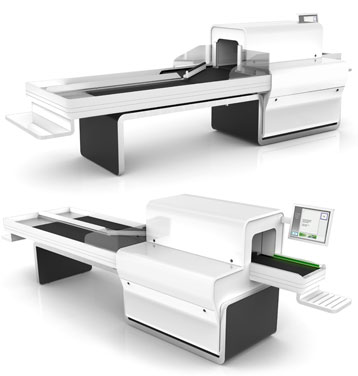
\includegraphics[width=0.3\textwidth]{scanflow.jpg}
  \end{center}
  \caption{A self-scan register}
  \label{fig:register}
\end{figure}

Axini has provided an IOSTS and an Adapter component for this case study. These are used for the testing and measurements.

\paragraph*{Stimuli and responses}
Appendix~\ref{app:scrp-specification} gives the most relevant parts of the specification document for this communication protocol. The entire specification is downloadable from the Twente University website\footnote{http://fmt.cs.utwente.nl/education/master/117/}. From this document, the following stimuli were designed:
\vspace{5px} \\
\begin{tabular}{lp{280px}} 
$\mathit{?SIGNON(id, password)}$ & Requests the register to sign on with the login and password given by $\mathit{id}$ and $\mathit{password}$\\
$\mathit{?SIGNOFF}$ & Requests the register to sign off\\
$\mathit{?OPEN(account)}$ & Opens the account given by $\mathit{account}$ or a new account if $\mathit{account}$ is not set\\
$\mathit{?ARTREG(barcode)}$ & Requests registration of an article, with $\mathit{barcode}$ representing its key \\
$\mathit{?STAMPREG}$ & Requests registration of loyalty points \\
$\mathit{?ARTID(barcode)}$ & Requests identification of an article, with $\mathit{barcode}$ representing its key\\
$\mathit{?ARTRET(barcode)}$ & Returns an article where $\mathit{barcode}$ is the article being returned \\
$\mathit{?CLOSE}$ & Closes the account\\
$\mathit{?ENDTOT}$ & Requests the end total of the registered articles\\
$\mathit{?TRANS(trans\_id)}$ & Inform the register that the payment was made, where $\mathit{tr\_method}$ represents the payment method, e.g. cash, credit card\\
$\mathit{?RECEIPT}$ & Requests the register return the receipt.\\
$\mathit{?PRINT(account)}$ & Requests the register to print additional information on the receipt for $\mathit{account}$\\
$\mathit{?IDLE}$ & Requests rounding-up of the account\\
$\mathit{?RESUME}$ & Requests the register to continue operation from an error state\\
$\mathit{?RHCOPY(account)}$ & Requests the register to print a hardcopy of a receipt for $\mathit{account}$\\
$\mathit{?RESETCR}$ & Requests the register to execute a reset \\
$\mathit{?GET(var\_name)}$ & Requests to get the value of a certain register variable represented by $\mathit{var\_name}$
\end{tabular}

The SCRP responses follow a coding scheme, much like the definition for FTP. The responses are a 3-digit status code, where each digit has a special significance. The first digit denotes the essence of the related action:
\begin{itemize}
\item 2yz Ok - Command has been accepted and the action is successfully completed. A new command may be issued.
\item 4yz Again - Command was not a accepted as a result of a temporary error condition. It is encouraged to request the same action again.
\item 5yz Fail - Command was not accepted as a result of a permanent error condition. It is discouraged to request the same action again.
\end{itemize}

The following function categories are encoded in the second digit:
\begin{itemize}
\item x0z Syntax - Command contained a syntax error (50z), or default indication if no other function category applies (10z, 20z, 30z, 40z)
\item x1z Information - Response related to access of information.
\item x2z Connection - Response related to connection/service.
\item x3z Account - Response related to account management.
\item x4z Transaction - Response related to (payment) transaction.
\item x5z Signing - Response related to sign on/off operations.
\item x6z Printing - Response related to receipt printing.
\end{itemize}

The third digit gives a finer gradation in each of the function categories, which leads to the complete list of responses:
\vspace{5px} \\
\begin{tabular}{ll}
$!201$ & Resumed operation\\ 
$!202$ & Cash Register restored\\ 
$!210(cr\_variable, cr\_value)$ & Gives the value of the variable $\mathit{cr\_variable}$\\ 
$!212(description,price)$ & Gives the description and price of a registered article\\ 
$!213(description,price)$ & Gives the description and price of a registered article\\ 
%$!214$ & <weight>:<weight\_price>:<price>:<barcode> CERTDATA\\ 
$!220$ & SCRP Service ready\\ 
$!221$ & SCRP Service terminating\\ 
$!230(endtotal)$ & Gives the end total for all registered articles.\\ 
$!231$ & Account opened\\ 
$!232$ & Article registered\\ 
$!233$ & Account idled\\ 
$!240$ & Transaction succeeded\\ 
$!250$ & Signed Off\\ 
$!251$ & Signed On\\ 
$!260$ & Data printed\\ 
$!261(html\_text)$ & Gives the receipt as HTML\\ 
$!450$ & Signing rejected\\ 
$!500$ & Unknown command\\ 
$!501$ & Syntax error\\ 
$!502$ & Command failed\\ 
$!503$ & Error state \\ 
$!510$ & No such variable\\ 
$!511$ & No such article\\ 
$!512$ & No stable weight\\ 
$!530$ & No such account\\ 
$!531$ & Invalid account state\\ 
$!540$ & No such transaction method\\ 
$!541$ & Busy transacting\\ 
$!542$ & Transaction failed\\ 
$!550$ & Not signed on\\ 
$!551$ & Authentication failed\\ 
$!560$ & CR-printing inactive \\
$!561$ & SFU-printing inactive
\end{tabular}

\paragraph*{Database testing} The available barcodes of articles are stored in a database. There are no stimuli to manipulate this database, nor is it feasible to let the model perform SQL statements to obtain barcodes. However, the model should know if an existing or non-existing barcode is given. The Adapter component is given access to the database and the stimuli with barcode as internaction variable are replaced by:
\vspace{5px}\\
\begin{tabular}{ll}
$\mathit{?ARTID\_EXIST}$ & Requests identification of an existing article \\
$\mathit{?ARTID\_NEXIST}$ & Requests identification of a non-existing article \\
%$ARTID\_WEIGHTED$,
$\mathit{?ARTRET\_EXIST}$ & Returns an existing article \\
$\mathit{?ARTRET\_NEXIST}$ & Returns a non-existing article \\
$\mathit{?ARTREG\_EXIST}$ & Requests the registration of an existing article \\
$\mathit{?ARTREG\_NEXIST}$ & Requests the registration of a non-existing article \\
$\mathit{?ARTREG\_REFUND}$ & Requests registration of a special type of article, the refund \\
$\mathit{?ARTREG\_LOYALTY}$ & Request registeration of a special type of aricle, the loyalty points \\
\end{tabular}

A similar abstraction is made for the $\mathit{account}$ interaction variable: 
\vspace{5px}\\
\begin{tabular}{lp{310px}}
$\mathit{?OPEN\_EXIST}$ & Opens an existing account \\
$\mathit{?OPEN\_NEXIST}$ & Opens a non-existing account \\
$\mathit{?PRINT\_EXIST}$ & Requests the register to print additional information on the receipt for an existing account \\
$\mathit{?PRINT\_NEXIST}$ & Requests the register to print additional information on the receipt for a non-existing account \\
$\mathit{?RHCOPY\_EXIST}$ & Requests the register to print the receipt for an existing account \\
$\mathit{?RHCOPY\_NEXIST}$ & Requests the register to print additional information on the receipt for a non-existing account \\
\end{tabular}
\vspace{5px} \\
And also for the login and password for the signing on: 
\vspace{5px}\\
\begin{tabular}{ll}
$\mathit{?SIGNON\_EXIST}$ & Sign on with a correct login/password \\
$\mathit{?SIGNON\_NEXIST}$ & Sign on with an incorrect login/password \\
\end{tabular}

\paragraph*{IOGG} Some selected rules of the IOGG of this communication protocol are shown in Figure~\ref{fig:gg-scrp}. In total the IOGG has 93 rules. They are downloadable from the Twente University website\footnote{http://fmt.cs.utwente.nl/education/master/117/}. Figure~\ref{fig:start-scrp} shows the initial graph. The $CR$ node is the cash register, the $SFU$ is the scanflow unit. The first node has the flag $\mathit{SS\_OFF}$ representing that the register is off. There is one account which can be in states idle, open, closed and transing. When the customer places items on the belt, a new account is opened. Figure~\ref{fig:open-account-request} shows the general request structure. As long as there is no request, a request can be sent. This rule requests the opening of an account. Figure~\ref{fig:open-account-success} shows the rule for giving a success response. The request node is deleted such that new request nodes can be created again. The rule checks if an account is not already opened and opens an idle account. Figure~\ref{fig:open-account-invalid} shows the rule for the error message received when an account is already opened. 

\begin{figure}[ht]
  \begin{center}
    \subfloat[The initial graph]{\label{fig:start-scrp}% To use this figure in your LaTeX document
% import the package groove/resources/groove2tikz.sty
%
% Special colors
\begin{tikzpicture}[
% Special color styles
scale=\tikzscale]
\node[node] (n0)  at (1.020, -1.065) {\ml{\textbf{CR}\\\textit{SS\_OFF}\\\textit{var\_1}\\state = "SS\_OFF"}};
\node[node] (n1)  at (2.420, -1.065) {\ml{\textbf{SFU}\\\textit{var\_2}\\var\_name = ""}};
\node[node] (n2)  at (1.035, -1.960) {\ml{\textbf{Account}\\\textit{AS\_IDLE}}};
\path[edge](n0.south -| 1.035, -1.960) -- node[lab]{has} (n2) ;
\userdefinedmacro
\end{tikzpicture}
\renewcommand{\userdefinedmacro}{\relax}
}\hspace{20px}
    \subfloat[The open account request rule]{\label{fig:open-account-request}% To use this figure in your LaTeX document
% import the package groove/resources/groove2tikz.sty
%
% Special colors
\begin{tikzpicture}[
% Special color styles
scale=\tikzscale]
\node[nacnode] (n1)  at (1.925, -1.555) {\ml{\textbf{Request}}};
\node[newnode] (n0)  at (1.915, -0.810) {\ml{\textbf{Request}\\\textit{open}}};
\node[node] (n2)  at (0.920, -1.125) {\ml{\textbf{CR}}};
\node[node] (n11)  at (2.970, -1.095) {\ml{\textbf{SFU}}};
\path[nacedge] (n1)  -- node[naclab]{to} (n2) ;
\path[newedge] (n0)  -- node[newlab]{to} (n2) ;
\path[nacedge] (n11)  -- node[naclab]{from} (n1) ;
\path[newedge] (n11)  -- node[newlab]{from} (n0) ;
\userdefinedmacro
\end{tikzpicture}
\renewcommand{\userdefinedmacro}{\relax}
}\\
    \subfloat[The open account success rule]{\label{fig:open-account-success}% To use this figure in your LaTeX document
% import the package groove/resources/groove2tikz.sty
%
% Special colors
\begin{tikzpicture}[
% Special color styles
scale=\tikzscale]
\node[delnode] (n3)  at (2.855, -0.770) {\ml{\textbf{Request}\\\textit{open}}};
\node[node] (n11)  at (2.850, -1.475) {\ml{\textbf{SFU}}};
\node[node] (n0)  at (1.705, -1.645) {\ml{\textbf{Account}\\{\color{\blue}\textit{$-$ AS\_IDLE}}\\{\color{\green}\textit{$+$ AS\_OPEN}}}};
\node[node] (n2)  at (1.695, -0.770) {\ml{\textbf{CR}\\\textit{SS\_ON}}};
\path[edge](n2.south -| 1.705, -1.645) -- node[lab]{has} (n0) ;
\path[deledge](n3.west |- 1.695, -0.770) -- node[dellab]{to} (n2) ;
\path[deledge](n11.north -| 2.855, -0.770) -- node[dellab]{from} (n3) ;
\userdefinedmacro
\end{tikzpicture}
\renewcommand{\userdefinedmacro}{\relax}
}\hspace{20px}
    \subfloat[The open account invalid rule]{\label{fig:open-account-invalid}% To use this figure in your LaTeX document
% import the package groove/resources/groove2tikz.sty
%
% Special colors
\begin{tikzpicture}[
% Special color styles
scale=\tikzscale]
\node[delnode] (n0)  at (2.005, -0.890) {\ml{\textbf{Request}\\\textit{open}}};
\node[node] (n11)  at (3.070, -0.875) {\ml{\textbf{SFU}}};
\node[nacnode] (n1)  at (1.010, -1.940) {\ml{\textbf{Account}\\\textit{AS\_IDLE}}};
\node[node] (n2)  at (0.990, -0.875) {\ml{\textbf{CR}\\\textit{SS\_ON}}};
\path[nacedge](n2.south -| 1.010, -1.940) -- node[naclab]{has} (n1) ;
\path[deledge](n11.west |- 2.005, -0.890) -- node[dellab]{from} (n0) ;
\path[deledge](n0.west |- 0.990, -0.875) -- node[dellab]{to} (n2) ;
\userdefinedmacro
\end{tikzpicture}
\renewcommand{\userdefinedmacro}{\relax}
}\\
    \subfloat[The not signed on error rule]{\label{fig:not-signed-on}% To use this figure in your LaTeX document
% import the package groove/resources/groove2tikz.sty
%
% Special colors
\begin{tikzpicture}[
% Special color styles
scale=\tikzscale]
\node[delnode] (n2)  at (2.185, -0.600) {\ml{\textbf{Request}\\{\color{\red}\textit{! signon}}}};
\node[node] (n1)  at (2.190, -1.235) {\ml{\textbf{SFU}}};
\node[node] (n0)  at (0.815, -0.610) {\ml{\textbf{CR}\\\textit{?[SS\_OFF,SS\_HALT]}}};
\path[deledge](n2.west |- 0.815, -0.610) -- node[dellab]{to} (n0) ;
\path[deledge](n1.north -| 2.185, -0.600) -- node[dellab]{from} (n2) ;
\userdefinedmacro
\end{tikzpicture}
\renewcommand{\userdefinedmacro}{\relax}
}\hspace{20px}
    \subfloat[The close account success rule]{\label{fig:close-account-success}% To use this figure in your LaTeX document
% import the package groove/resources/groove2tikz.sty
%
% Special colors
\begin{tikzpicture}[
% Special color styles
scale=\tikzscale]
\node[node] (n6)  at (2.820, -0.725) {\ml{\textbf{SFU}}};
\node[node] (n5)  at (0.595, -0.770) {\ml{\textbf{CR}\\\textit{SS\_ON}}};
\node[node] (n0)  at (0.605, -1.735) {\ml{\textbf{Account}\\{\color{\blue}\textit{$-$ AS\_OPEN}}\\{\color{\green}\textit{$+$ AS\_CLOSED}}}};
\node[delnode] (n8)  at (1.695, -0.760) {\ml{\textbf{Request}\\\textit{close}}};
\path[deledge](n6.west |- 1.695, -0.760) -- node[dellab]{from} (n8) ;
\path[deledge](n8.west |- 0.595, -0.770) -- node[dellab]{to} (n5) ;
\path[edge](n5.south -| 0.605, -1.735) -- node[lab]{has} (n0) ;
\userdefinedmacro
\end{tikzpicture}
\renewcommand{\userdefinedmacro}{\relax}
}
  \end{center}
  \caption{A few selected rules from the IOGG of the Scanflow Cash Register Protocol}
  \label{fig:gg-scrp}
\end{figure}

For all these rules, the $CR$ node has to have the flag $\mathit{SS\_ON}$ representing the register to be signed on. Figure~\ref{fig:not-signed-on} shows the response to a request when the register is not signed on. Apart from the signon request, no other request is allowed in this state. Figure~\ref{fig:close-account-success} shows the rule closing the account.

\paragraph*{IOSTS} The IOSTS of the system as created by Axini is shown in a seperate document, also downloadable from the Twente University website\footnotemark[\value{footnote}]. It has 907 locations, 1302 switch relations and 2 location variables.